\documentclass[12pt]{report}
\usepackage{graphicx} % Required for inserting images
\usepackage[a4paper, margin=2.5cm]{geometry}
\graphicspath{{images/}}

\usepackage[utf8]{inputenc}
\usepackage[T1]{fontenc}
\usepackage{float} % here for H placement parameter
\usepackage{subcaption}

\usepackage{filecontents}
\usepackage[
    firstinits=true, % render first and middle names as initials
    useprefix=true,
    maxcitenames=3,
    maxbibnames=99,
    style=authoryear,
    dashed=false, % re-print recurring author names in bibliography
    natbib=true,
    url=false
]{biblatex}

\title{CMP5352 Report - TITLE NEEDED}
\author{Lewis Higgins - Student ID 22133848}
\date{April 2024}

\usepackage[outputdir=./auxil]{minted}

\renewbibmacro*{volume+number+eid}{%
    \printfield{volume}%
%  \setunit*{\adddot}% DELETED
    \setunit*{\addnbspace}% NEW (optional); there's also \addnbthinspace
    \printfield{number}%
    \setunit{\addcomma\space}%
    \printfield{eid}}
\DeclareFieldFormat[article]{number}{\mkbibparens{#1}}

\addbibresource{report.bib}

% Use single quotes around titles:
\usepackage[british]{babel}
\usepackage{csquotes}

\usepackage{hyperref}

\hypersetup{
    colorlinks=true,
    linkcolor=black,
    filecolor=magenta,
    urlcolor=blue,
    citecolor=black,
}


\urlstyle{same}


% To prevent "Chapter N" display for each chapter
\usepackage[compact]{titlesec}
\usepackage{wasysym}
\usepackage{import}

\titlespacing*{\chapter}{0pt}{-2cm}{0.5cm}
\titleformat{\chapter}[display]
{\normalfont\bfseries}{}{0pt}{\Huge}

\newcommand\blfootnote[1]{
    \begingroup
    \renewcommand\thefootnote{}\footnote{#1}
    \addtocounter{footnote}{-1}
    \endgroup
}

\usepackage{fancyhdr}
\usepackage{calc}
\pagestyle{fancy}

\setlength\headheight{37pt}

\renewcommand{\chaptermark}[1]{%
    \markboth{#1}{}}

\lhead{Lewis Higgins - ID 22133848~~~~~~~~~~~~~~~
\includegraphics[width=1.75cm]{bcu logo}}
\fancyhead[R]{\leftmark}

\usepackage{xcolor}
\definecolor{mintedBG}{rgb}{0.95, 0.95, 0.95}

\begin{document}
    \pagecolor{yellow} % Change in final

    \makeatletter
    \begin{titlepage}
        \begin{center}
            
\includegraphics[width=0.7\linewidth]{bcu logo}\\[4ex]
            {\large \bfseries  \@title }\\[2ex]
            {\large \bfseries  DRAFT VERSION }\\[2ex]
            {\@author}\\[30ex]
            {Word count: XXXX}\\[20ex]
        \end{center}
    \end{titlepage}
    \makeatother
    \thispagestyle{empty}
    \newpage

    \pagecolor{white}

    \begin{abstract}
        text

        text

        text

    \end{abstract}

    \setcounter{page}{0} % Page counter bullshit to make it ACTUALLY start from 1

    \tableofcontents
    \thispagestyle{empty}

    \chapter*{Introduction}\label{ch:introduction}
    \addcontentsline{toc}{chapter}{Introduction}
    \markboth{Introduction}{}

    Text text text

    Text text text

    \pagebreak

    aaa

    \chapter*{Motivation and objectives}\label{ch:sec1}
    \addcontentsline{toc}{chapter}{Motivation and objectives}
    \markboth{Motivation and objectives}{}


%   \inputminted[linenos=true, breaklines=true, bgcolor=mintedBG, stripall=true]{r}{lab4.R}
    \begin{minted}[]{r}
library(ggplot2)
ggplot(diamonds, aes(x = carat, fill = color)) +
        geom_histogram(bins = 30)
\end{minted}

\begin{figure}[H]

{\centering 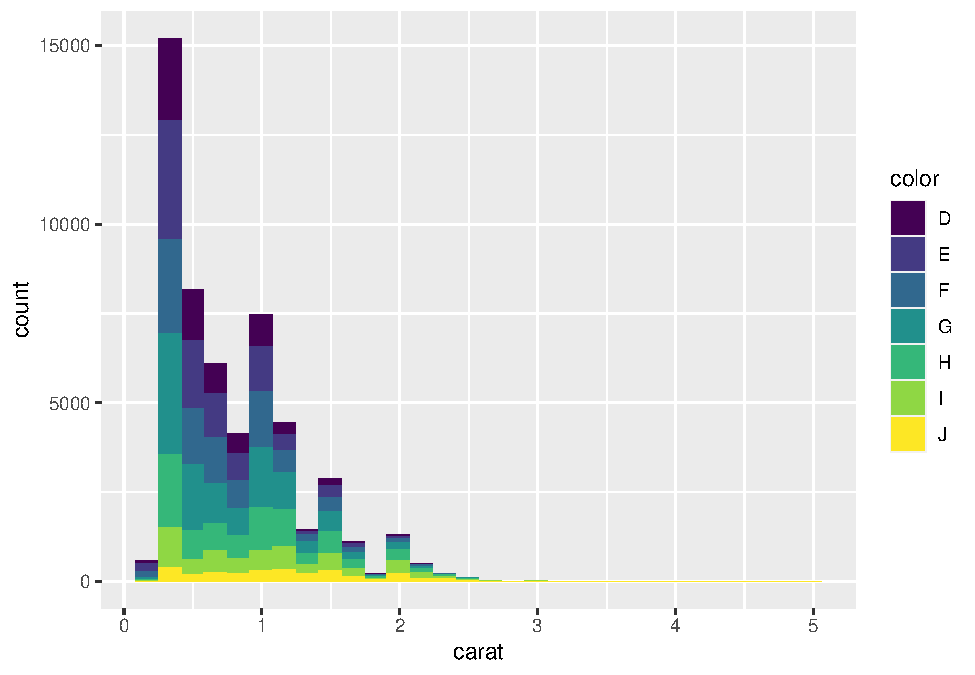
\includegraphics[width=0.75\linewidth]{../images/figs/chunk1-1} 

}

\caption{\label{fig:fig1}Plot 1}\label{fig:chunk1}
\end{figure}

Figure \ref{fig:fig1} shows that\ldots{}

\pagebreak

\begin{minted}[]{r}
ggplot(diamonds, aes(x = carat, y = price)) +
    geom_point(aes(color = cut)) +
    geom_smooth()
\end{minted}

\begin{figure}[H]

{\centering 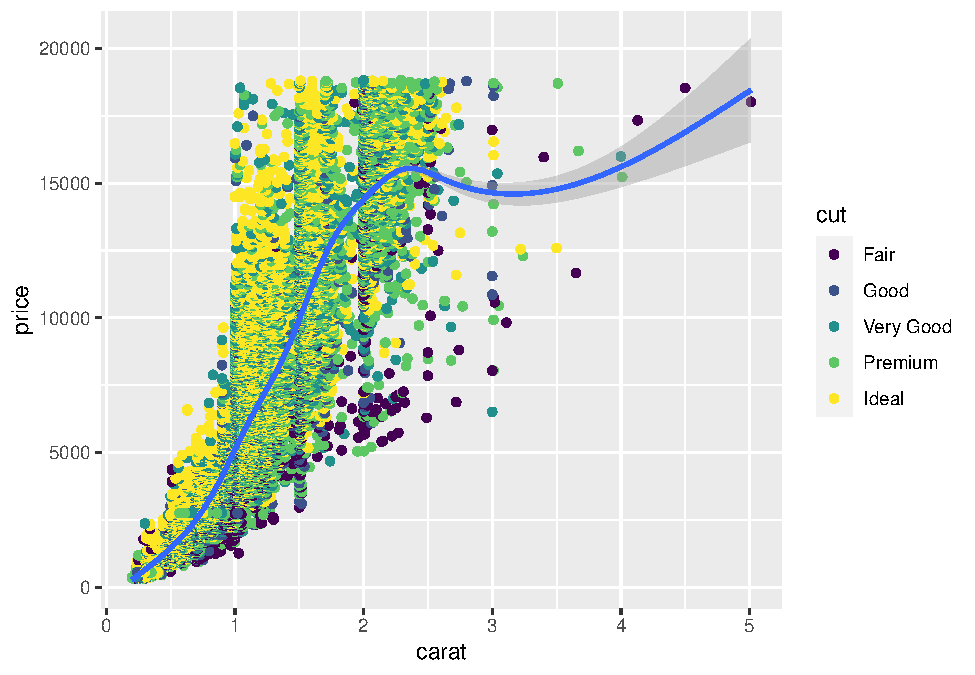
\includegraphics[width=0.75\linewidth]{../images/figs/chunk2-1} 

}

\caption{\label{fig:fig2}Plot 1}\label{fig:chunk2}
\end{figure}

Figure \ref{fig:fig2} instead shows that\ldots{}


    \pagebreak


    \chapter*{Experimental results}\label{ch:sec2}
    \addcontentsline{toc}{chapter}{Experimental results}
    \markboth{Experimental results}{}

    text text text

text text text

    \chapter*{Summary \& conclusion}\label{ch:sec3}
    \addcontentsline{toc}{chapter}{Summary and conclusion}
    \markboth{Summary and conclusion}{}

    text text text

text text text


\end{document}